
% \mm{We don't need to include Figure~\ref{fig:edp4} as its average results are already in the previous figure.}
% \begin{figure*}[t]%
% 	\centering
% 	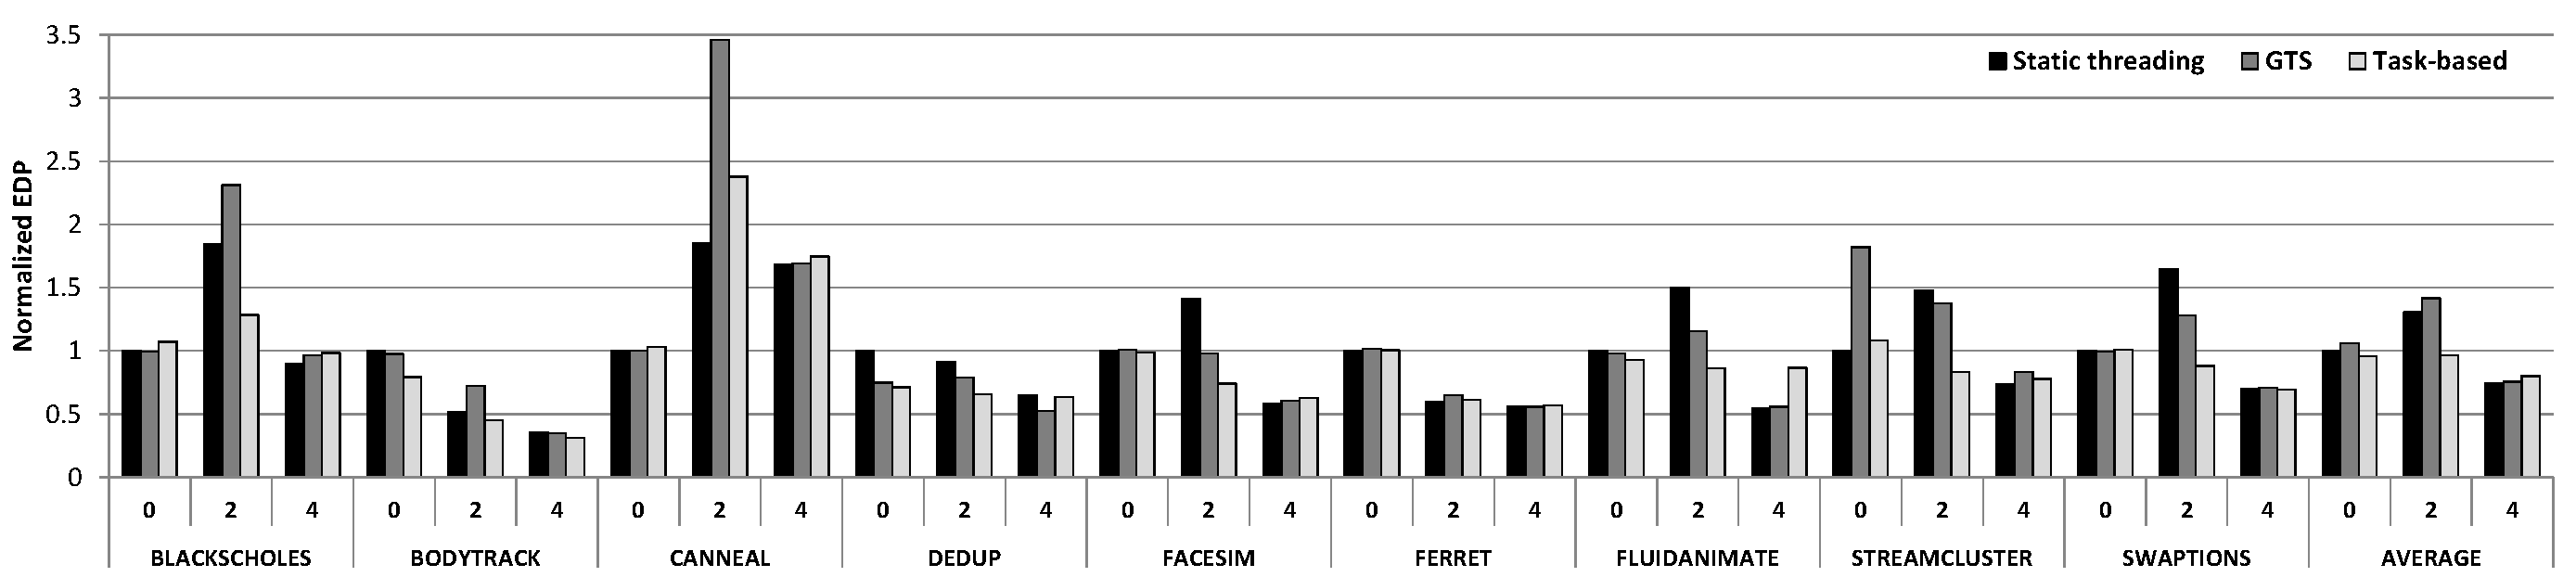
\includegraphics[width=1.0\textwidth]{figures/edp4.pdf}
% 	\vspace{-0.3cm}
% 	\caption{Normalized EDP on a 4-core system with 0, 2, and 4 big cores. Results are normalized with respect to static-threading EDP results with 4 little cores.}
% 	%\caption{Performance improvements on a big.LITTLE processor with different $(F,N)$ configurations, where $F$ is the total number of big cores and $N$ the total number of cores. Results are normalized to running on four little cores with pinned Pthreads.}%
% 	\label{fig:edp4}%
% \end{figure*}


% \begin{figure*}[t]%
% 	\centering
% 	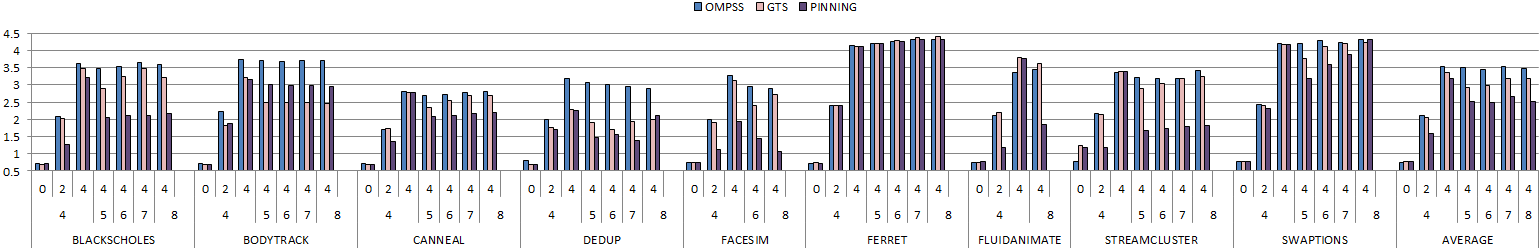
\includegraphics[width=1.0\textwidth]{figures/power-parsec}
% 	\vspace{-0.3cm}
% 	\caption{Average power consumption on a big.LITTLE processor with different $(F,N)$ configurations, where $F$ is the total number of big cores and $N$ the total number of cores.}%
% 	\label{fig:all-power}%
% \end{figure*}
% 
% \begin{figure*}[t]%
% 	\centering
% 	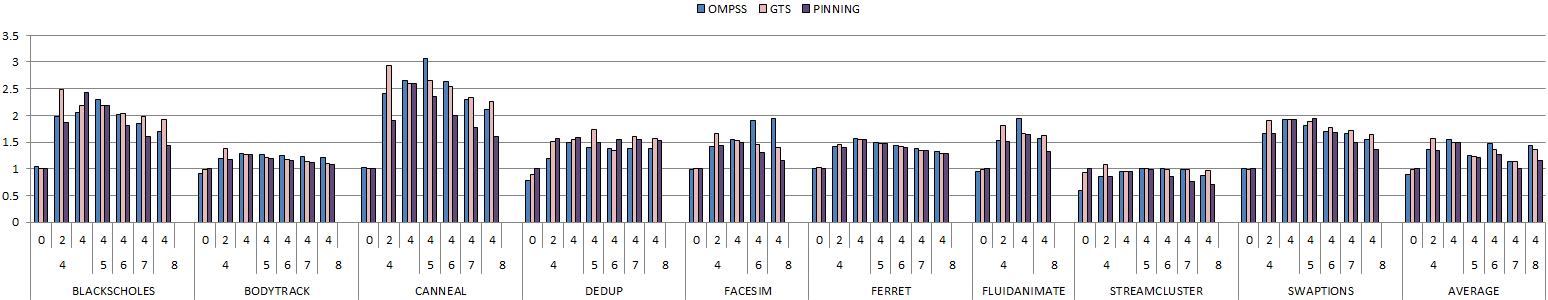
\includegraphics[width=1.0\textwidth]{figures/energy-parsec}%
% 	\vspace{-0.3cm}
% 	\caption{Energy consumption on a big.LITTLE processor with different $(F,N)$ configurations, where $F$ is the total number of big cores and $N$ the total number of cores. Results are normalized to running on four little cores with pinned Pthreads.}%
% 	\label{fig:all-energy}%
% \end{figure*}
% 
% 
% 
% \begin{figure*}[t]%
% 	\centering
% 	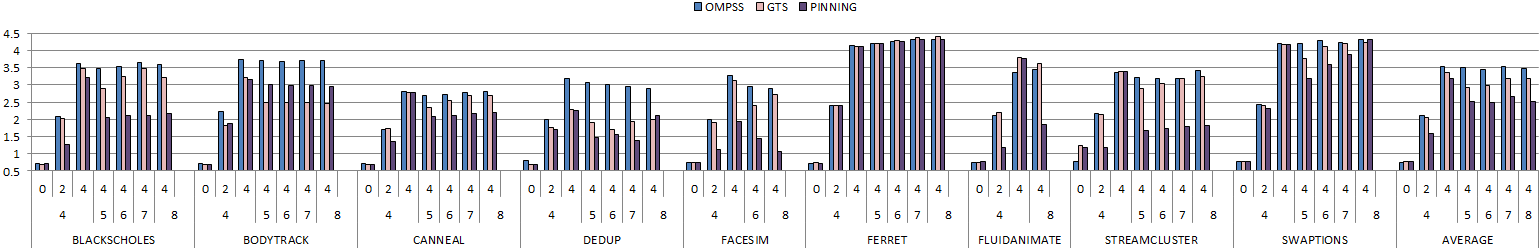
\includegraphics[width=1.0\textwidth]{figures/power-parsec}
% 	\vspace{-0.3cm}
% 	\caption{Average power consumption on a big.LITTLE processor with different $(F,N)$ configurations, where $F$ is the total number of big cores and $N$ the total number of cores.}%
% 	\label{fig:all-power}%
% \end{figure*}
% 
% \begin{figure*}[t]%
% 	\centering
% 	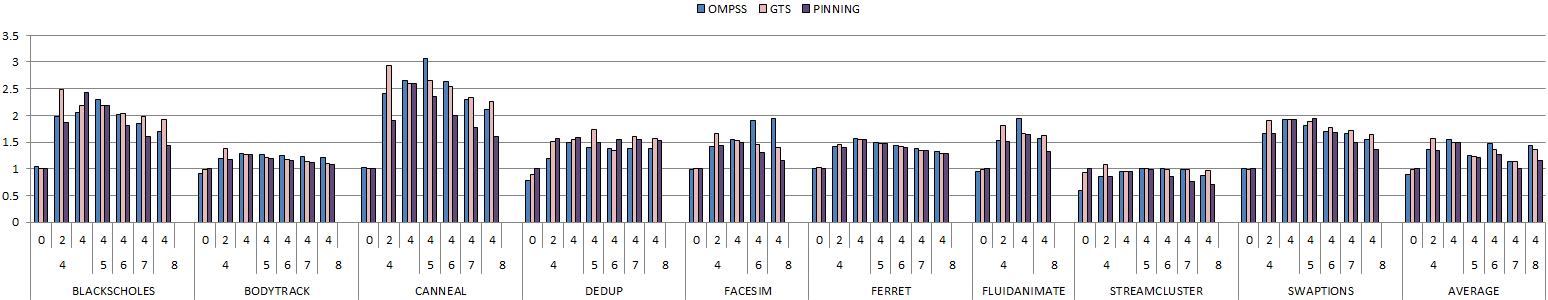
\includegraphics[width=1.0\textwidth]{figures/energy-parsec}%
% 	\vspace{-0.3cm}
% 	\caption{Energy consumption on a big.LITTLE processor with different $(F,N)$ configurations, where $F$ is the total number of big cores and $N$ the total number of cores. Results are normalized to running on four little cores with pinned Pthreads.}%
% 	\label{fig:all-energy}%
% \end{figure*}



We measure execution time, power, energy and EDP of nine 
applications from the PARSEC benchmark suite~\cite{Bienia:PhD2011}. We compare these metrics for 
three different scheduling approaches:
\begin{itemize}
\item \textit{Static threading}: scheduling decisions are made at the application level. The OS is not allowed to migrate threads between the clusters of big and little cores. 
\item \textit{GTS}\footnote{We choose to evaluate GTS instead of CS and IKS because it is the most advanced scheduling approach supported in the Linux kernel.}: dynamic coarse-grained OS scheduling 
using the GTS scheduler integrated in the Linux kernel~\cite{samsung, ARM} using the default 
PARSEC benchmarks. 
\item \textit{Task-based}: dynamic fine-grained scheduling at the runtime level with the task-based implementations of the benchmarks provided in PARSECSs~\cite{Chasapis:TACO2016}.
\end{itemize}


%%%%%%%%%%%%%%%%%%%%%%%%%%%%%%%%%%%%%%%%%%
%%%%%%%%%%%%%%%%%%%%%%%%%%%%%%%%%%%%%%%%%%
\subsection{Exploiting Parallelism in AMCs}
\label{sec:eval:A}

% \mm{This section should focus on identifying the problems that current applications have on an asymmetric/heterogeneous multicore. For example, static scheduling, homogeneous domain/workload partition. More dynamic applications, will scale better (bodytrack, dedup, ferret, freqmine, vips).}

This section examines the opportunities and challenges that current AMCs offer to emerging parallel applications. With this objective, we first evaluate a system with a constant number of four cores, changing the level of asymmetry to evaluate the characteristics of each configuration. In these experiments, all applications run with the original parallelization strategy that relies on the user to balance the application (\emph{Static threading}). We also evaluate the OS-based dynamic scheduling (\emph{GTS}) and the task-based runtime dynamic scheduling (\emph{Task-based}) for the same applications. 
% Figure~\ref{fig:ideal} shows the ideal speedup of the system for all the different combination of big and little cores. 
The system configurations evaluated in this section are:
i)~Four little cores (\texttt{0+4}); ii)~Two big and two little cores (\texttt{2+2}); and iii)~Four 
big cores (\texttt{4+0})

% \begin{itemize}
% \item Four little cores (\texttt{0+4})
% \item Two big and two little cores (\texttt{2+2})
% \item Four big cores (\texttt{4+0})
% \end{itemize}
For these configurations, Figure~\ref{fig:speedup4} shows the speedup of the PARSEC benchmarks with respect to running on a single little core. Figure~\ref{fig:power4} reports the average power dissipated on the evaluated platform. Finally, Figure~\ref{fig:energy4} shows the total energy consumed per application for the same configurations. Energy results are normalized to the energy measured with four little cores (higher values imply higher energy consumptions). Average EDP results are also included in this figure.

Focusing on the average performance results, we notice that all approaches perform similarly for the homogeneous configurations. 
Specifically, applications obtain the best performance on the configuration~\emph{4+0}, with an average speedup of 9.5$\times$ over one little core. 
When using four little cores, an average speedup of 3.8$\times$ is reached for all approaches. 
This shows that all the approaches are effective for this core count. 
In the configuration~\emph{2+2}, \emph{Static threading} slightly improves performance (5.0$\times$ speedup), while \emph{GTS} and \emph{Task-based} reach significantly higher speedups: 5.9$\times$ and 6.8$\times$, respectively.
\begin{figure*}[t]%
	\centering
	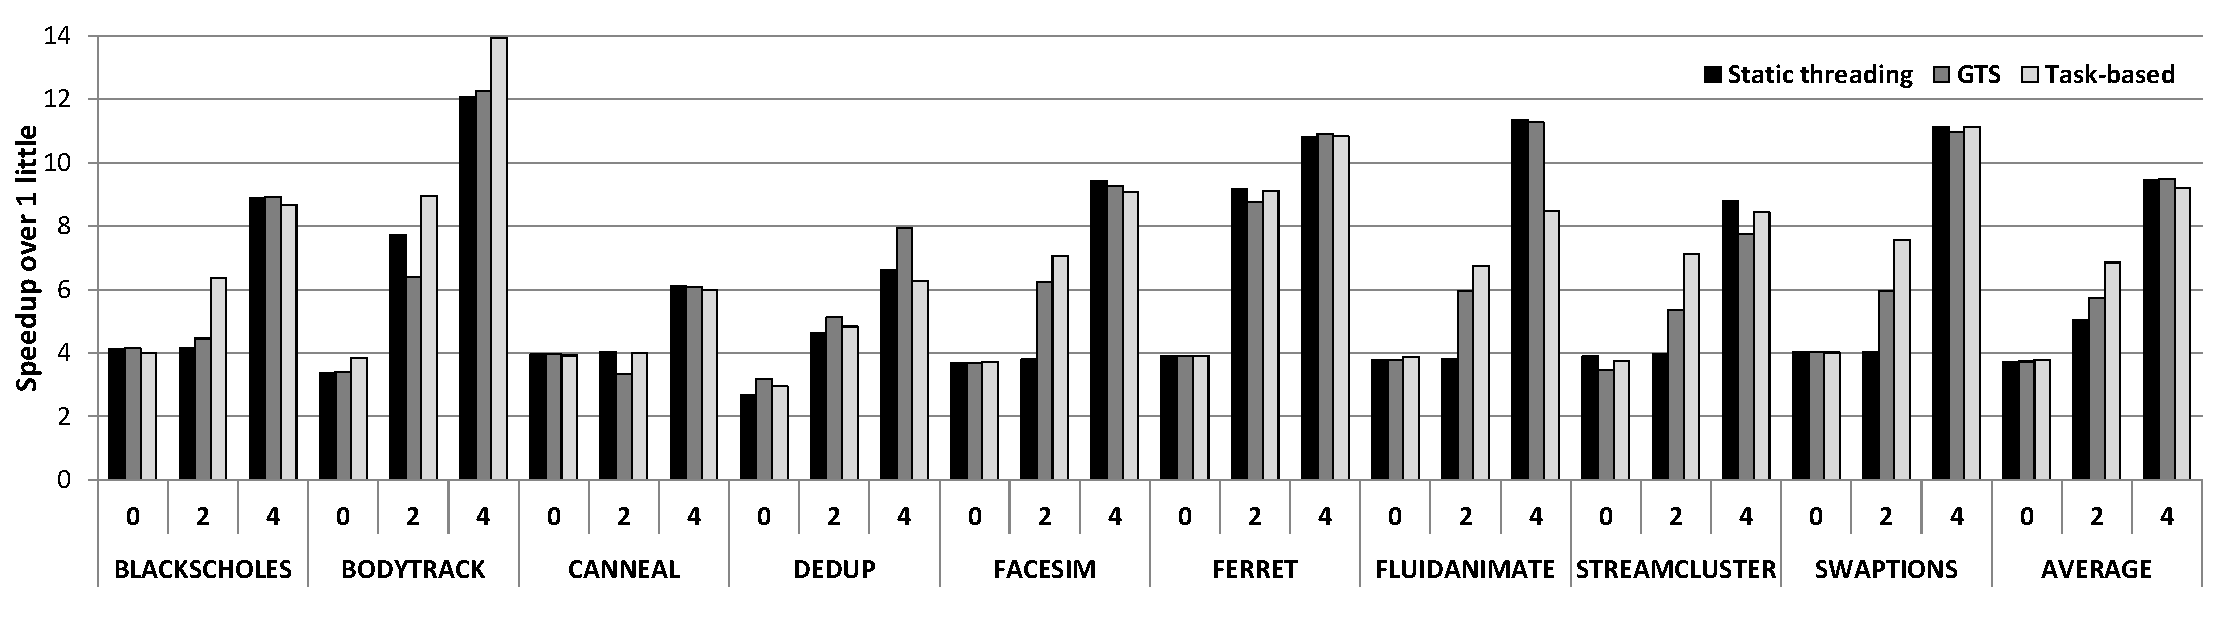
\includegraphics[width=1.0\textwidth]{figures/speedup-4_new.pdf}
	\vspace{-0.5cm}
	\caption{Execution time speedup over 1 little core for systems that consist of 4 cores in 
		total with 0, 2 and 4 big cores. Different schedulers at the application (\textit{static 
			threading}), OS  (\textit{GTS}) and runtime (\textit{task-based}) levels are considered.}
	%\caption{Performance improvements on a big.LITTLE processor with different $(F,N)$ configurations, where $F$ is the total number of big cores and $N$ the total number of cores. Results are normalized to running on four little cores with pinned Pthreads.}%
	\label{fig:speedup4}%
\end{figure*}
\begin{figure*}[t]%
	\centering
	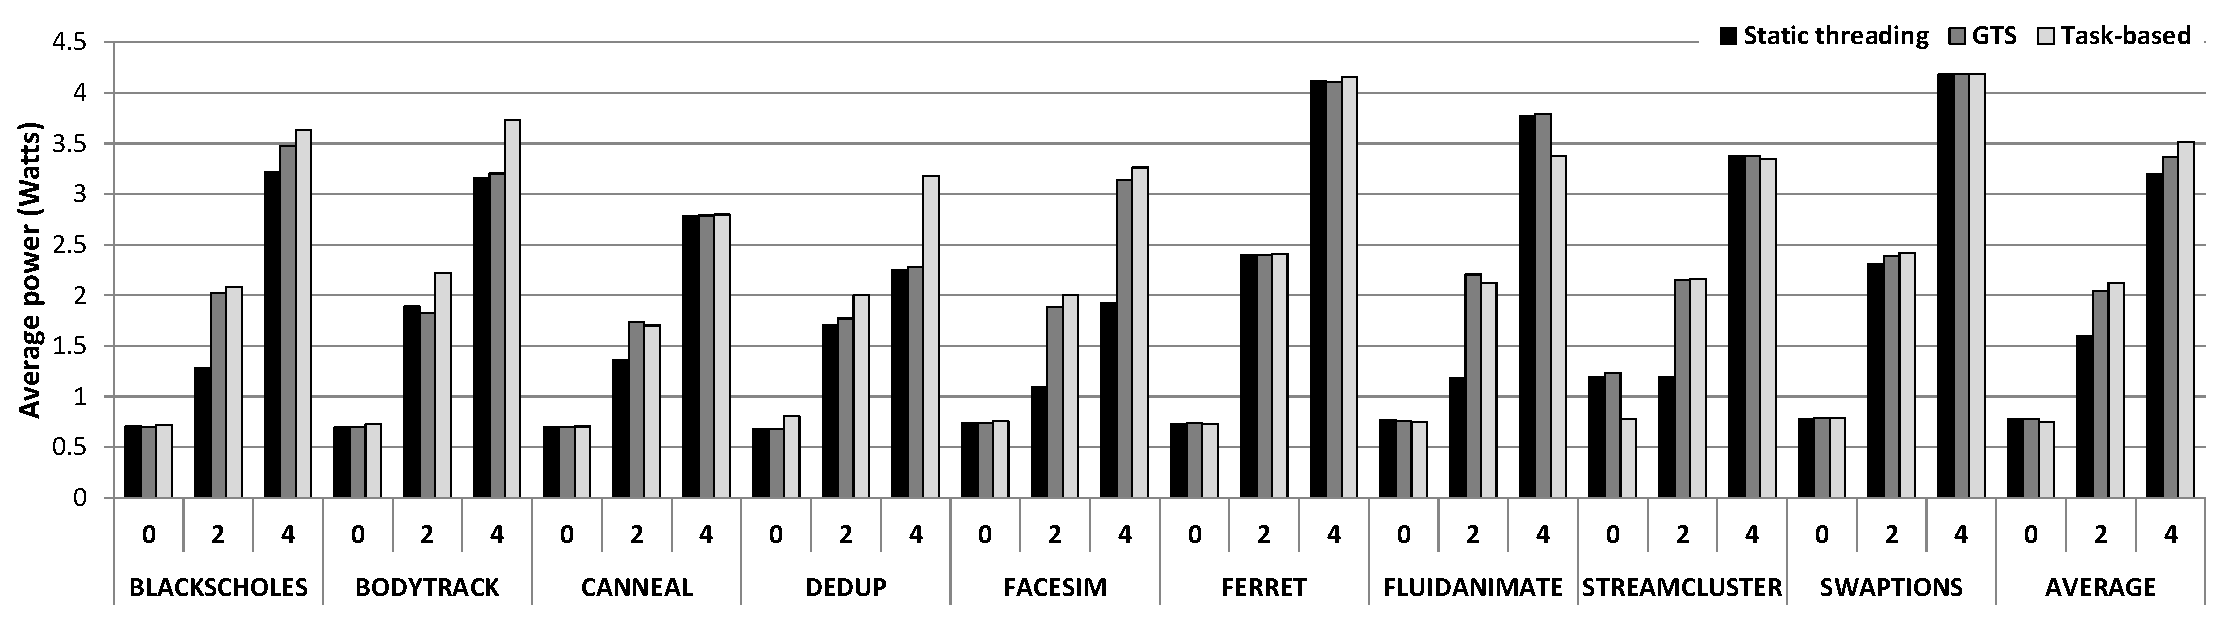
\includegraphics[width=1.0\textwidth]{figures/power4_new.pdf}
	\vspace{-0.5cm}
	\caption{Average power measurements on a 4-core system with 0, 2, and 4 big cores.}
	%\caption{Performance improvements on a big.LITTLE processor with different $(F,N)$ configurations, where $F$ is the total number of big cores and $N$ the total number of cores. Results are normalized to running on four little cores with pinned Pthreads.}%
	\label{fig:power4}%
\end{figure*}
\begin{figure*}[!h]%
	\centering
	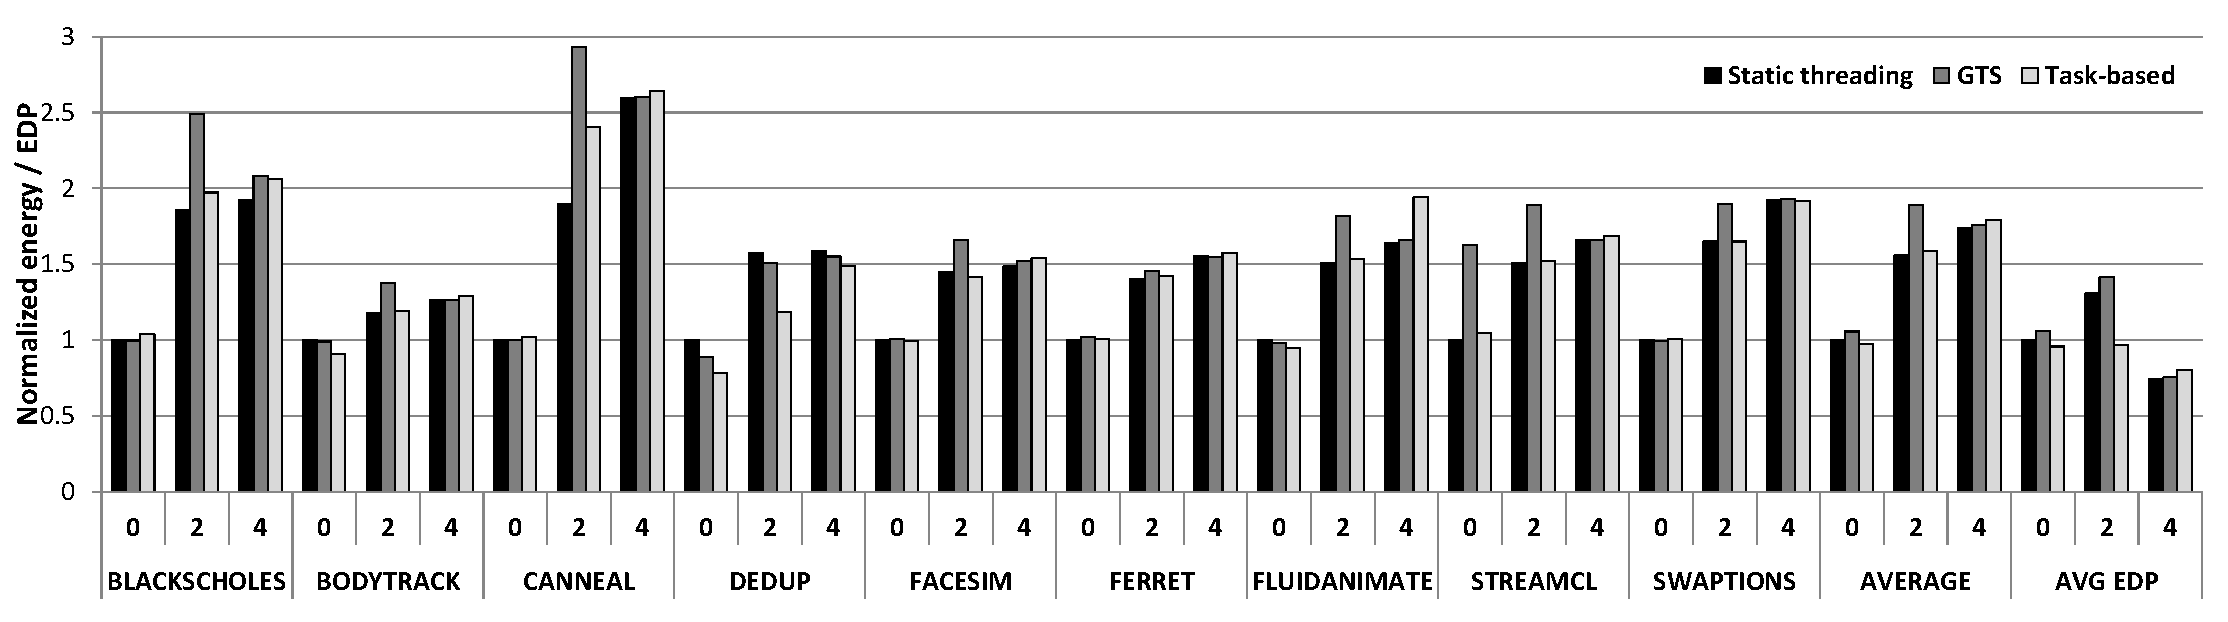
\includegraphics[width=1.0\textwidth]{figures/energy_EDP-4_new.pdf}
	\vspace{-0.5cm}
	\caption{Normalized energy consumption and average EDP on a 4-core system with 0, 2, and 4 big cores. Static threading on 4 little cores is the baseline in both cases. }
	%\caption{Performance improvements on a big.LITTLE processor with different $(F,N)$ configurations, where $F$ is the total number of big cores and $N$ the total number of cores. Results are normalized to running on four little cores with pinned Pthreads.}%
	\label{fig:energy4}%
\end{figure*}

Contrarily, in terms of power and energy, the most efficient configuration is running with four little cores, as the performance ratio between the different cores is inversely proportional to the power ratio~\cite{Greenhalgh2011}. On average, all the approaches reach a power dissipation of 0.75W for the \texttt{0+4} configuration, while \emph{Task-based} reaches 3.5W for the \texttt{4+0} configuration which is the one with the highest average power dissipation. In configuration \texttt{2+2}, average energy values for \emph{Static threading} and \emph{Task-based} are nearly the same, as the increase in power from 1.6W to 2.1W is compensated by a significant improvement in performance of 30\%.

Finally, in terms of EDP using the four big cores is the optimal, as the performance improvements compensate the increase in total energy. 
In configuration \texttt{2+2}, \emph{Task-based} achieves the same EDP results as in \texttt{0+4}, but with 81\% better performance. 
For the asymmetric configuration, \emph{Task-based} achieves the best performance-energy combination since its dynamic scheduling is effectively utilizing the little cores. 

%\texttt{0+4} reaches a power dissipation of 0.75W with all approaches, while \emph{Task-based} reaches 3.5W in configuration \texttt{4+0}.

%\kc{Consider removing this paragraph? It just mentions the obvious results that reviewers are complaining about...} Thus, if the number of cores remains constant, the best configuration in terms of performance and EDP corresponds to a symmetric configuration with big cores (e.g. \texttt{4+0}), while in terms of power and energy the best configuration corresponds to a symmetric configuration with little cores (e.g. \texttt{0+4}). 
% From the average energy-delay product (EDP) results in Figure~\ref{fig:energy4} we can approximate the configuration that achieves the highest performance with the best possible energy consumption. The configuration with the lowest EDP is the one with four big cores (\texttt{4+0}) since all the scheduling approaches manage to compensate the additional energy consumption with the speedup that can be achieved on this set-up. However, it is interesting to note that for the asymmetric configuration the \emph{Task-based} approach achieves the best combination of performance and energy since its dynamic scheduling approach is effectively utilizing the little cores. 

Next, we focus on the obtained results per benchmark. 
For applications with an extensive use of barriers (blackscholes, facesim, fluidanimate, streamcluster and swaptions) or with a memory intensive pattern (canneal), the extra computational power offered by the big cores in configuration \texttt{2+2} is not exploited. 
As a result with \emph{Static threading} performance is only slightly improved by 1\% on average when moving from \texttt{0+4} to the \texttt{2+2} configuration. 
This slight improvement comes at the cost of much more power and energy consumption (79\% and 77\% respectively).
These results are explained three-fold: i) load is distributed homogeneously among threads in some 
applications; ii) extensive usage of barriers force big cores to wait until little cores reach the 
barrier; and iii) high miss rates in the last-level cache cause frequent pipeline stalls and prevent 
to fully exploit the computational power of big cores. 
To alleviate these problems, the programmer should develop more advanced parallelization strategies that could benefit from AMCs, as performed in the remaining applications, or rely on dynamic scheduling at OS or runtime levels.

\textcolor{blue}{
\textbf{R1Q6:} GTS is a suitable alternative for barrier-synchronized applications (blackscholes, facesim, fluidanimate, streamcluster and swaptions) when asymmetry is introduced. 
GTS enhances performance as it is dynamically migrating the threads around the cores depending on the CPU utilization.
Thus it is expected that performance will increase compared to static threading for the asymmetric configuration. 
For these applications, the \emph{task-based} approach further improves GTS for the asymmetric configuration.
This is because \emph{task-based} schedules tasks among threads which is much more efficient than scheduling threads among cores.
}

The three remaining applications are parallelized using a pipeline model (bodytrack, dedup, and ferret)  with queues for the data-exchange between pipeline stages and application-specific dynamic load balancing mechanisms designed by the programmer.
As a result, \emph{Static threading} with these applications benefits from the extra computational power of the big cores in the configuration \texttt{2+2}. 
\textcolor{blue}{
\textbf{R1Q6:} Since \emph{Static threading} can already maintain load balance for these applications due to their implementation, there is no need for dynamic thread migration that is introduced by GTS.
}
%The advanced load balancing mechanisms introduced in these applications are not needed in the \emph{Task-based} code; 
\textcolor{blue}{
\textbf{R1Q4:} Using the \emph{task based} approach, the code of the application is simplified allowing the application to express even more parallelism as the runtime system automatically allows the overlapping of the different pipeline stages. 
This can be verified by the fact that bodytrack obtains higher performance with the \emph{task based} approach even for the symmetric configurations.
}
On the asymmetric configuration, \emph{Task-based} further improves the obtained performance, reaching a 13\% average improvement over \emph{GTS}. 
Clearly, these applications benefit in performance by the increased number of big cores, while power and energy are increasing since the big cores are effectively utilized.

%In these applications, all the approaches clearly outperform configuration \texttt{0+4}, while still increasing power and energy, as now all cores are busy (not only the little ones).

%the parallel regions to overlap more aggressively different stages of the pipeline. As a result, \emph{Task-based} further improves the obtained performance, reaching a 13\% average speedup over \emph{GTS}. In these applications, all the approaches clearly outperform configuration \texttt{0+4}, while still increasing power and energy, as now all cores are busy (not only the little ones).

Generally, relying on the programmer to statically schedule asymmetric configurations does not report good results, as it is very hard to predict the system's behavior at application-level. 
Only applications that implement advanced features with user-level schedulers and load balancing techniques, can benefit from asymmetry, at the cost of programmability effort.
Relying on the OS scheduler is a suitable alternative without code modifications, but relying on the runtime to dynamically schedule tasks on the asymmetric processor achieves much better performance, power and energy results.

%the developer did not consider it when designing the parallelization technique. When applications implement advanced features with user-level schedulers and load balancing techniques, applications can benefit from asymmetry, of course at the cost of programmability effort. A suitable alternative consists in relying on the OS system or the runtime to dynamically schedule tasks into the asymmetric processor, reaching much better performance, power and energy results in these systems.


%To estimate the best configuration when taking into account both performance and energy efficiency we have to 


%Relying on the programmer to benefit from asymmetry does not report good results, as the developer did not consider it when designing the parallelization technique. When applications implement advanced features with user-level schedulers and load balancing techniques, applications can benefit from asymmetry, of course at the cost of programmability effort. A suitable alternative consists in relying on the OS system or the runtime to dynamically schedule tasks into the asymmetric processor, reaching much better performance, power and energy results in these systems.

%, power or energy corresponds to a homogeneous configuration with in-order cores (power and energy) or big cores (performance). 

%In general relying on the programmer to benefit from asymmetry does not report good results, as the developer did not consider it when designing the parallelization technique. When applications implement advanced features with user-level schedulers and load balancing techniques, applications can benefit from asymmetry, of course at the cost of programmability effort. A suitable alternative consists in relying on the OS system or the runtime to dynamically schedule tasks into the asymmetric processor, reaching much better performance, power and energy results in these systems.
\iffalse
\mm{Figure~\ref{fig:energy4} also shows the average normalized results for EDP. In this case, lower is better. I didn't comment these results yet. With this metric, Task-based on 2+2 is as good as the others in 0+4 while we obtain better performance. This is interesting, but I'm not sure if it adds much with respect to the already presented numbers.}

\mm{I haven't commented much the results with the GTS scheduler. Maybe we should extend this part. Next, I put some sentences that might be useful, although I don't know where to put them.}

As described in Section~\ref{sec:scheduling}, the Global Task Scheduler (GTS) migrates tasks between cores in order to balance the load in the different cores of the heterogeneous processor. 

For fork-join + homogeneous load, the scheduler should be very effective, reaching the performance results of OmpSs. However, it is unaware of what it is moving around, which means that it might move a thread that is idle to a big core...

Consequently, for some benchmarks, the OS is making decisions without coordinating with the application scheduler and can worsen the performance. This should be the case of the applications with advanced load balancing techniques, but I still don't know if we will see this behavior.
\fi

% \begin{figure*}[t]%
% 	\centering
% 	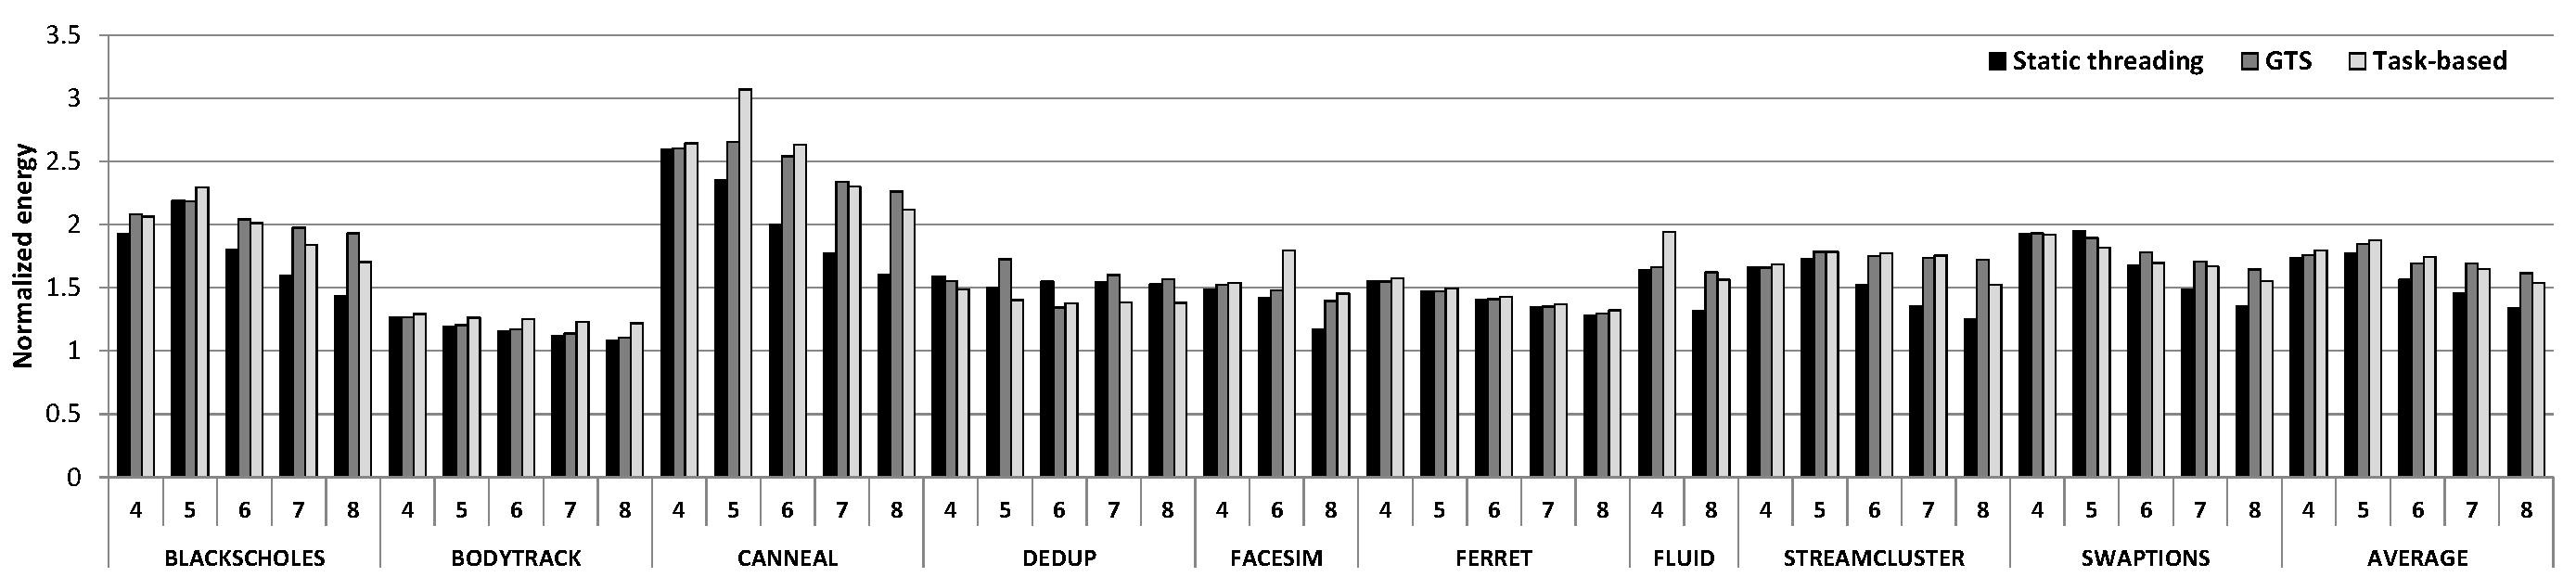
\includegraphics[width=1.0\textwidth]{figures/energy-4plus.pdf}
% 	\vspace{-0.5cm}
% 	\caption{Normalized energy consumption with respect to 4-little-static-threading energy consumption, when running on 4 to 8 cores and 4 of them are big}
% 	%\caption{Performance improvements on a big.LITTLE processor with different $(F,N)$ configurations, where $F$ is the total number of big cores and $N$ the total number of cores. Results are normalized to running on four little cores with pinned Pthreads.}%
% 	\label{fig:energy4plus}%
% 	\vspace{-0.3cm}
% \end{figure*}

% \begin{figure*}[t]%
% 	\centering
% 	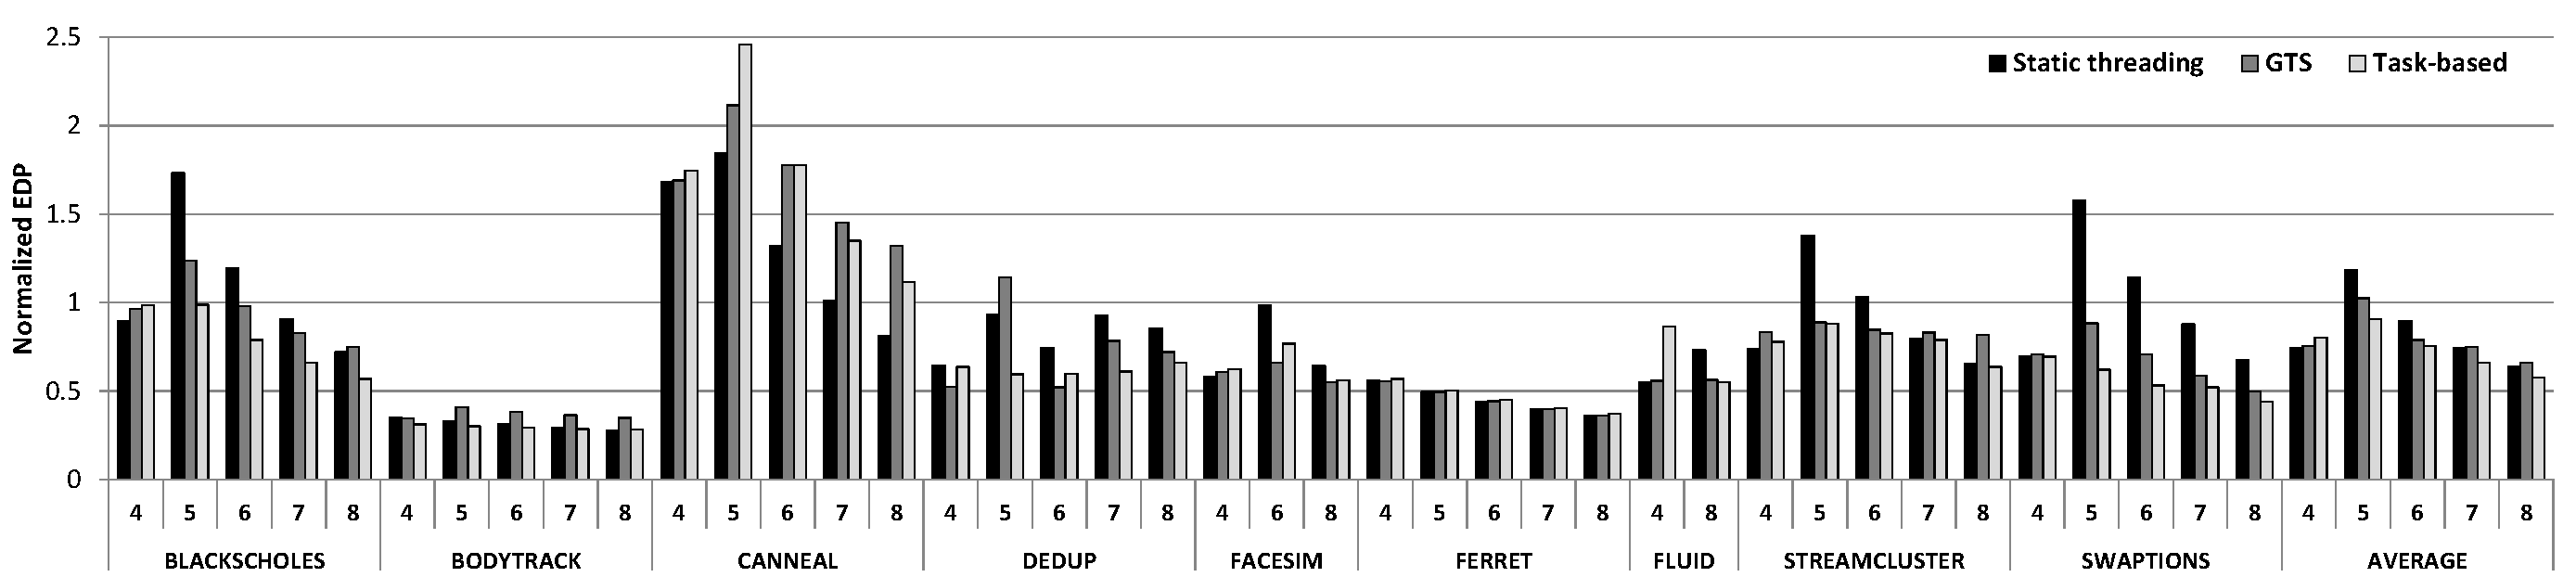
\includegraphics[width=1.0\textwidth]{figures/edp4plus.pdf}
% 	\vspace{-0.3cm}
% 	\caption{Normalized EDP when running on 5, 6, 7, or 8 cores and 4 of them are big}
% 	%\caption{Performance improvements on a big.LITTLE processor with different $(F,N)$ configurations, where $F$ is the total number of big cores and $N$ the total number of cores. Results are normalized to running on four little cores with pinned Pthreads.}%
% 	\label{fig:edp4plus}%
% \end{figure*}


%%%%%%%%%%%%%%%%%%%%%%%%%%%%%%%%%%%%%%%%%%
%%%%%%%%%%%%%%%%%%%%%%%%%%%%%%%%%%%%%%%%%%
\subsection{Adding Little Cores to an SMC}
\label{sec:eval:B}
In the following experiments, we explore if an application running on a symmetric multi-core (SMC) with big cores can benefit from adding small cores that help in its execution. Having more computational resources increases the ideal speedup a parallel application can reach, but it also introduces challenges at application, runtime and OS level. 
Thus, we examine how many small cores have to be added to the system to compensate the cons of having to deal with AMCs.

To evaluate this scenario, we explore configurations \texttt{4+0}, \texttt{4+1}, \texttt{4+2}, \texttt{4+3} and \texttt{4+4}. In these experiments, the number of big cores remains constant (four), while the number of little cores increases from 0 to 4. First we focus on the average results of speedup, power, energy and EDP, shown in Figure~\ref{fig:averages4plus}.

The speedup chart of Figure~\ref{fig:averages4plus} shows that \emph{Static threading} does not benefit from adding little cores to the system.
In fact, this approach brings an average 6\% slowdown when adding four little cores for execution (\texttt{4+4}).
This is a result of the static thread scheduling; because the same amount of work is assigned to each core, when the big cores finish the execution of their part, they become idle and under-utilized. 
GTS achieves a limited speedup of 8\% with the addition of four little cores to the \texttt{4+0} configuration. The addition of a single little core brings a 22\% slowdown (from \texttt{4+0} to \texttt{4+1}) and requires three additional little cores to reach the performance of the symmetric configuration (\texttt{4+3}).  Finally, the \emph{Task-based} approach always benefits from the extra computational power as the runtime automatically deals with load imbalance. Performance improvements keep growing with the additional little cores, reaching an average improvement of 15\% over the symmetric configuration when 4 extra cores are added. 
%An interesting observation is that according to the ideal speedup (Equation~\ref{eq.ideal} and Figure~\ref{fig:ideal}), the average ideal performance increase when moving from the \texttt{4+0} configuration to the \texttt{4+4} is 33\%, considering that the average performance ratio is 2.96$\times$ as shown in Table~\ref{tab:parsec}. Thus, the task-based approach achieves almost half of this theoretical ideal performance.

%the execution time speedup of the PARSEC benchmarks with respect to running in a single in-order core. 
%When looking at the average results, it is very interesting to see that the \emph{Static threading} approach clearly fails to benefit from the extra in-order cores. Even with four extra cores (configuration \texttt{4+4}), an average 15\% slowdown is obtained. \emph{GTS} also suffers a significant performance reduction when adding an extra little core (22\% slowdown) and requires three additional little cores to match the performance of the symmetric configuration. With an additional extra core, \emph{GTS} reaches an average 5\% speedup over the symmetric configuration. 


\begin{figure*}[t]%
	\centering
	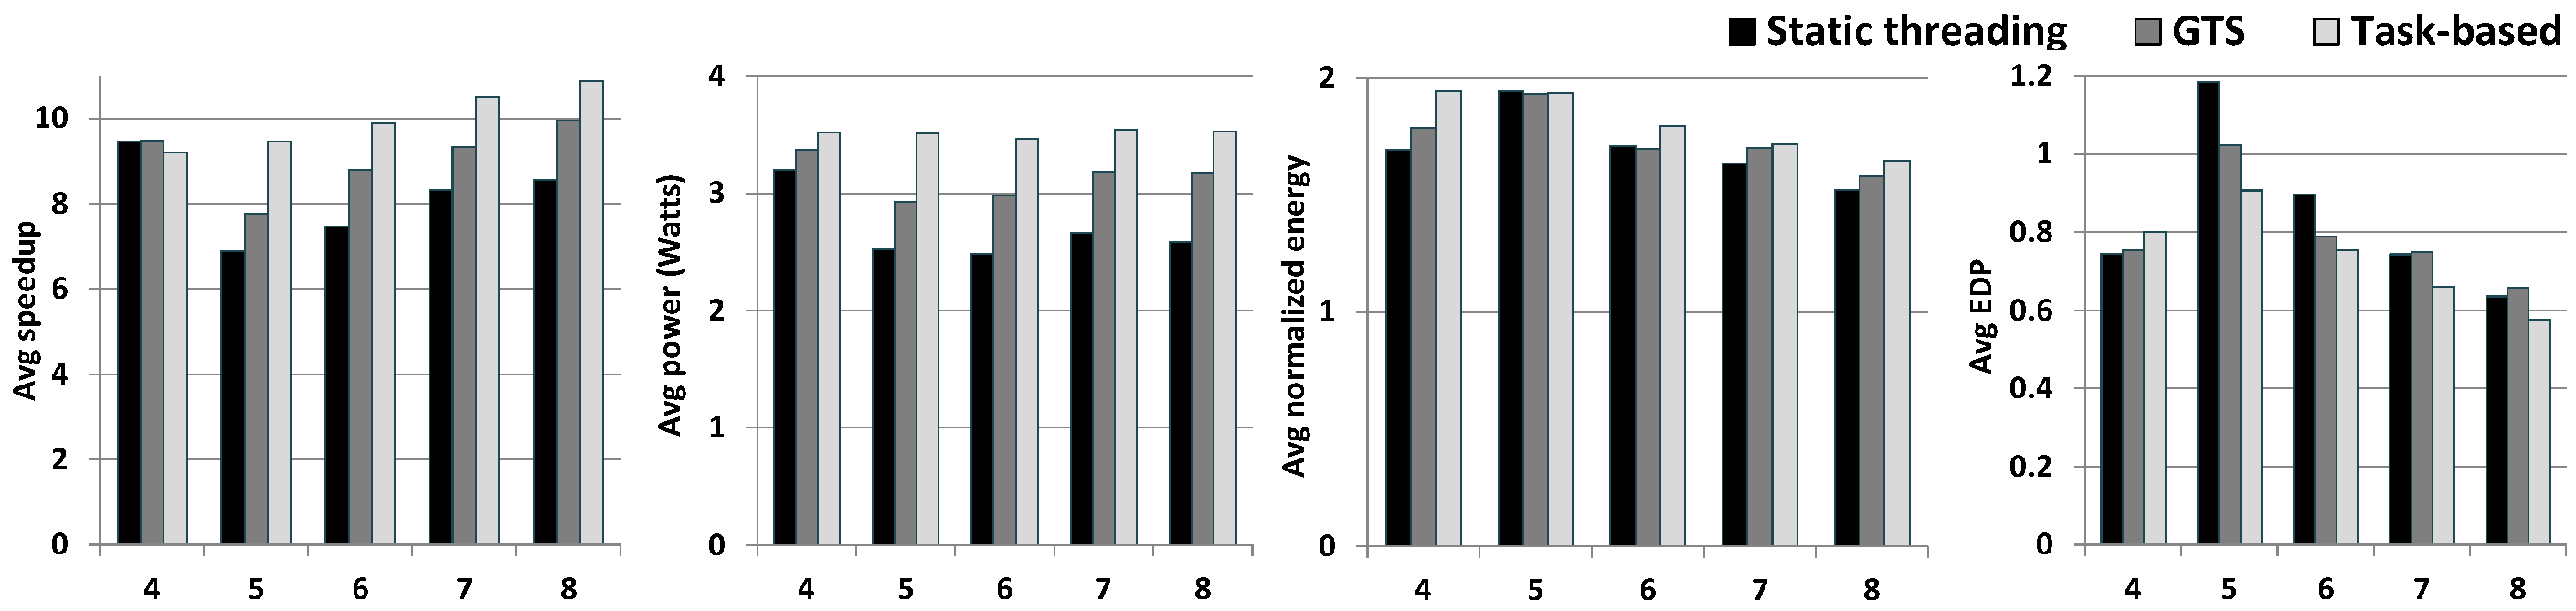
\includegraphics[width=\textwidth]{figures/averages_4plus_new.pdf}
	\vspace{-0.5cm}
	\caption{Average results when running on 4 to  8 cores with 4 of them big. Speedup is over 1 little core. Static threading on 4 little cores is the baseline of energy consumption and EDP}
	%\caption{Performance improvements on a big.LITTLE processor with different $(F,N)$ configurations, where $F$ is the total number of big cores and $N$ the total number of cores. Results are normalized to running on four little cores with pinned Pthreads.}%
	\label{fig:averages4plus}%
	\vspace{-0.3cm}
\end{figure*}

%In contrast, the \emph{Task-based} approach always benefits from the extra computational power as the runtime automatically deals with load imbalance. Performance improvements keep growing with the additional little cores, reaching an average improvement of 16\% over the symmetric configuration when 4 extra cores are added. Please, note that according to Table~\ref{tab:parsec} the performance ratio between big and little cores is 2.96$\times$, which means that the ideal speedup when adding 4 little cores to a system with 4 big cores is 1.33$\times$ ($\frac{2.96\cdot 4 + 4}{2.96\cdot 4}$). Thus, the \emph{Task-based} approach reaches half of the potential speedup on this asymmetric platform.

The power chart of Figure~\ref{fig:averages4plus} shows oppositional benefits among the three approaches. We can see that \emph{Static threading} and \emph{GTS} benefit from asymmetry, effectively reducing average power consumption.
\emph{Static threading} reduces power consumption when moving from the \texttt{4+0} to the \texttt{4+4} system by 23\% while \emph{GTS} does so by 6.2\%.
On the other hand, the \emph{task-based} approach keeps the big cores busy for most of the time so it maintains the average power nearly constant.


%In terms of power, the tradeoffs completely change. As shown in Figure~\ref{fig:power4plus}, \emph{Static threading} and \emph{GTS} always benefit from asymmetry, effectively reducing average power consumption. On average in configuration \texttt{4+4}, \emph{Static threading} and \emph{GTS} reduce power 23\% and 6.2\%, respectively, with respect to the symmetric multi-core. In contrast, the \emph{Task-based} approach always has all big cores busy and maintains overall power nearly constant. 

%In terms of energy, the third chart of Figure~\ref{fig:averages4plus} shows that the \emph{Static threading} significantly reduces energy consumption by 31\% when moving from \texttt{4+0} to the \texttt{4+4} configuration. As shown in the previous section, little cores are more energy efficient than big cores, at the cost of reduced performance. In the case of \emph{GTS} and \emph{Task-based}, at least two extra cores are needed to reduce energy. 
% In configuration \texttt{4+4}, energy is reduced by 31\% for \emph{Static threading}, 9.3\% for \emph{GTS}, and 16\% for \emph{Task-based}. Consequently, we can state that asymmetry reduces overall energy consumption, although the best configuration in terms of energy consists in using only four little cores.


The reduction in power, results to reduced average energy in the case of 
\emph{Static threading} in configuration \texttt{4+4}, as shown on the energy chart of 
Figure~\ref{fig:averages4plus}. As discussed in Section~\ref{sec:eval:A}, little cores are more energy 
efficient than big cores, at the cost of reduced performance. In all the approaches, at least two 
extra little cores are needed to reduce energy. In configuration \texttt{4+4}, energy is reduced by 
14\% for \emph{Static threading}, 15\% for \emph{GTS}, and 16\% for \emph{Task-based}. Consequently, we can state that asymmetry reduces overall energy consumption.
%, although the best configuration in terms of energy consists in using only four little cores (as average normalized energy is always above 1).

%--- ADD EDP results comments on average EDP
To see the impact on both performance and energy efficiency we plot the average EDP on the 
rightmost chart of Figure~\ref{fig:averages4plus}. In this chart the lower values are the better. The \emph{task-based} approach is the one that has the best performance-energy 
combination for the asymmetric configurations since it maintains the lowest EDP for all cases. 
\emph{Static threading} manages to reduce the average EDP by 6\% while \emph{GTS} and \emph{task 
based} approaches do so by 24\% and 36\% respectively.
%---
\begin{figure*}[t]%
	\centering
	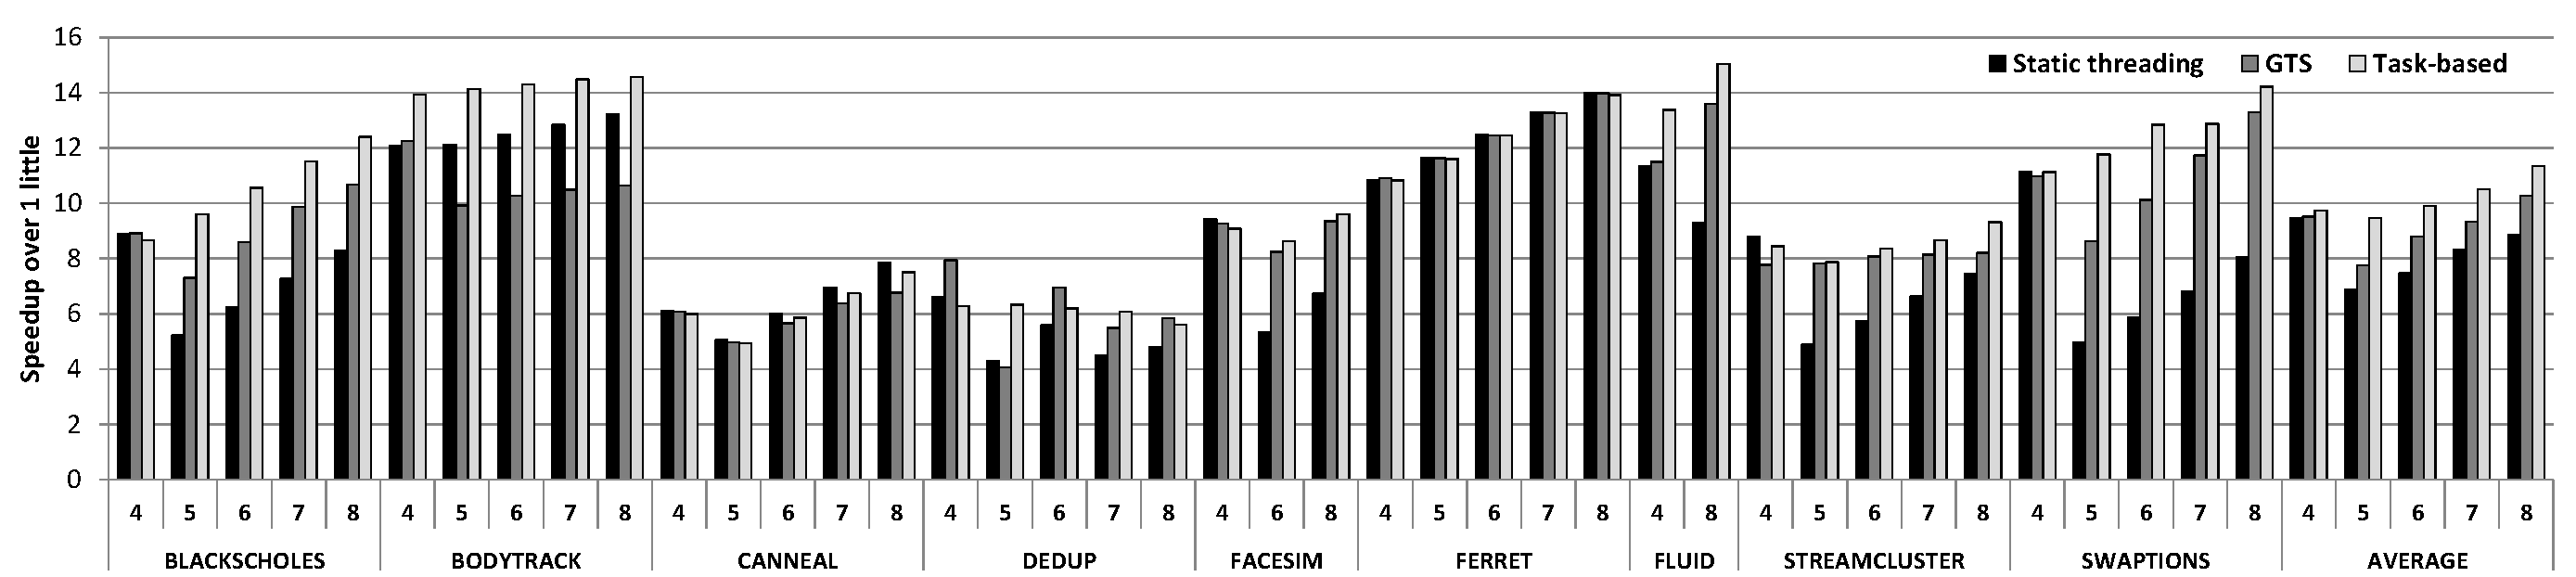
\includegraphics[width=1.0\textwidth]{figures/speedup-4plus.pdf}
	\vspace{-0.5cm}
	\caption{Speedup over 1 little core when running on 4 to 8 cores and 4 of them are big}
	%\caption{Performance improvements on a big.LITTLE processor with different $(F,N)$ configurations, where $F$ is the total number of big cores and $N$ the total number of cores. Results are normalized to running on four little cores with pinned Pthreads.}%
	\label{fig:speedup4plus}%
\end{figure*}
\begin{figure*}[t]%
	\centering
	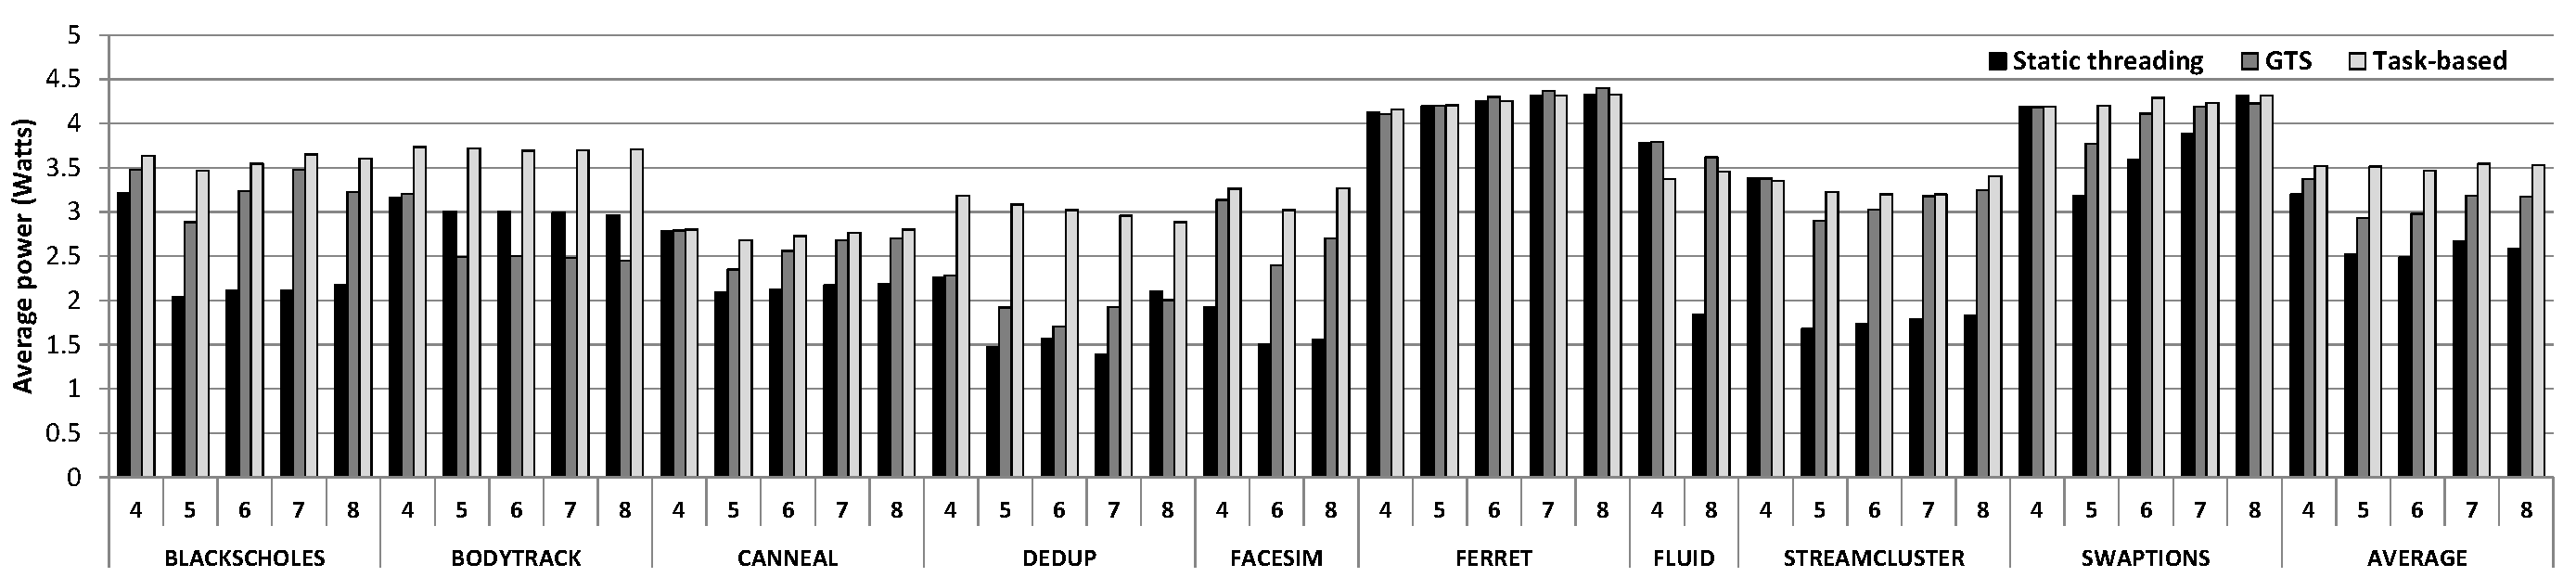
\includegraphics[width=1.0\textwidth]{figures/power4plus.pdf}
	\vspace{-0.5cm}
	\caption{Average power when running on 4 to 8 cores and 4 of them are big}
	%\caption{Performance improvements on a big.LITTLE processor with different $(F,N)$ configurations, where $F$ is the total number of big cores and $N$ the total number of cores. Results are normalized to running on four little cores with pinned Pthreads.}%
	\label{fig:power4plus}%
\end{figure*}

Figure~\ref{fig:speedup4plus} shows a more detailed exploration of the performance results. 
As Table~\ref{tab:parsec} shows, the applications with barrier synchronization are blackscholes, facesim, fluidanimate, streamcluster and swaptions. 
For these applications the most efficient system configuration with the \emph{Static threading} approach is the \texttt{4+0}. 
Little cores increase execution time due to load imbalance effects. 
\textcolor{blue}{
	\textbf{R1Q10:} \emph{GTS} and \emph{task-based} approaches overcome these issues by scheduling the load to the appropriate resources. 
	The differences in the improvement of the \emph{task based} and GTS solutions for these applications relies on the nature of each application and its parallel implementation.
	For example, swaptions, benefits more from the \emph{task based} and \emph{GTS} approaches than streacmluster.  
	This is because the task graph of streamcluster presents multiple small parallel regions that are spawned and synchronized. 
	Due to the multiple synchronization points, \emph{GTS} and \emph{task-based} cannot increase performance of streamcluster as much. 
	Contrarily, swaptions has less synchronization points, thing that allows GTS and task-based to exploit asymmetry during its longer parallel regions.
}
%we mention this later
%Since the big cores reach barriers earlier, power is reduced for these applications, as shown in Figure~\ref{fig:power4plus}. 
%Energy reduction is less significant with a few extra little cores as the performance degradation is higher, but as the number of little cores increases, energy is reduced. 



Applications with more advanced load balancing techniques like pipelined parallelism (bodytrack, dedup and ferret), benefit of the asymmetric hardware and balance the load among all the cores. 
\textcolor{blue}{As a result, the performance of \emph{Static threading} approach does not degrade when adding little cores as in the previous set of applications.
}
%As a result, performance improves as we increase the number of little cores. 
In the case of bodytrack, \emph{GTS} reduces performance by 15\% when 
adding four little cores. 
We attribute this to the cost of the thread migration from one core to the 
other in contrast to the \emph{Static threading} approach that does not add such overheads.
\textcolor{blue}{
\emph{Task based} approach also avoids these overheads and improves the performance of bodytrack by efficiently scheduling the tasks among threads.
}
%\kc{Please check this and let me know if makes sense. I had to write a comment for bodytrack.} 
In the case of dedup, results show more variability. This benchmark is very I/O intensive and, depending on the type of core that executes these I/O operations, performance drastically changes. In order to deal with this problem, a smarter dynamic scheduling mechanism would be required. 
%Ferret, obtains similar results with all approaches as its implementation is efficient with all scheduling approaches.
Finally, canneal does not scale according to its ideal speedup reported on Figure~\ref{fig:ideal} as it has a memory intensive pattern that limits performance.

Figure~\ref{fig:power4plus} shows the average power. The barrier-synchronized applications (blackscholes, facesim, fluidanimate, streamcluster and swaptions) reduce power because 
of their imbalance; since big cores have long idle times with the \emph{Static threading} approach, they do not dissipate the same power as \emph{GTS} and \emph{Task-based}.
%the big cores reach barriers earlier and remain idle, so power is reduced for the \emph{Static threading} approach compared to \emph{GTS} and \emph{Task-based}. 
For pipeline-parallel applications, both bodytrack and ferret maintain nearly the same 
power levels among the configurations for each scheduling approach. Dedup is an exception, as the 
results highly depend on the core that executes the aforementioned I/O operations. Yet, the 
effect of the lower power for \emph{Static threading} is observed in all the benchmarks and is because the big cores are under-utilized. %' long idle times.

%Each one of the pipeline-parallel applications (bodytrack, dedup, ferret) maintains nearly the same power levels among the configurations for each scheduling approach. 

%In these cases, the big cores do not remain as  Canneal also spends constant power among system configurations for the same reason.

%, while power consumption remains approximately the same. Consequently, total energy is reduced benefits in these asymmetric configurations.

%When focusing on the individual results per benchmark, the best configuration in terms of performance for applications with barriers (blackscholes, facesim, fluidanimate, streamcluster and swaptions) and with a memory intensive pattern (canneal) is \texttt{4+0}. Simple in-order cores increase execution time due to load imbalance effects. Since the big cores reach barriers earlier, power is reduced as a result for these applications, as shown in Figure~\ref{fig:power4plus}. Energy reduction is less significant with few extra little cores as the performance degradation is too high, but as the number of little cores increases, energy is reduced. 



%For applications with advanced load balancing techniques (bodytrack, dedup, and ferret), the application can take advantage of the asymmetric hardware and schedule load in all the cores. As a result, performance improves while we increase the number of little cores, while power consumption remains approximately the same. Consequently, total energy is reduced benefits in these asymmetric configurations. In the case of bodytrack, \emph{GTS} is having problems and a 20\% reduction in performance is obtained. \mm{Any idea why?}. In the case of dedup, results show more variability. This benchmark is very I/O intensive and, depending on which core executes these I/O operations, performance drastically changes. In oder to deal with this problem, a smarter dynamic scheduling mechanism would be required.
\textcolor{blue}{
\section*{Discussion}
\textbf{R1Q11: }Sections~\ref{sec:eval:A} and~\ref{sec:eval:B} explored the potential of different scheduling approaches when used on various workloads on an AMC. 
It was proven that current applications are not ready to utilize an AMC and that adding little cores to an SMC with big cores presents significant challenges for the application, OS and runtime developers. 
Little cores increase load imbalance and can degrade performance as a result. 
}

\textcolor{blue}{
A dynamic OS scheduler such as \emph{GTS} helps in mitigating load imbalance, providing an average performance increase of 10\%.
Barrier synchronized applications benefit more from the \emph{GTS} approach as the applications with more sophisticated scheduling techniques can utilize the little cores more efficiently even with \emph{Static threading}.
\emph{Task based} approach offers the optimal performance results for all types of workloads.
It improves \emph{Static threading} by 20\% on average by effectively balancing the load among big and little cores.
}

%Relying on the programmer to deal with this asymmetry is complex, but a dynamic OS scheduler such as \emph{GTS} helps in mitigating these problems, providing an average performance increase of 10\%. 
%However, the optimal performance results are obtained with the \emph{Task-based} approach, as they improve static threading by 23\% on average. 
In terms of power and energy, the AMC provides significant benefits, although the SMC with little cores remains the most energy-efficient configuration. 
\textcolor{blue}{
\textbf{R1Q9:} This is attributed to the differences of the designs of the big and little cores; little cores have been optimized for power efficiency while the design of the big cores targets higher performance levels at the cost of higher energy consumption.
}
The answer to the question of which system configuration provides the best power-performance balance, can be found on the average EDP chart of Figures~\ref{fig:energy4} and \ref{fig:averages4plus}, and is the use of the entire 8-core system with the \emph{Task based} approach.

%%%%%%%%%%%%%%%%%%%%%%%%%%%%%%%%%%%%%%%%%%
%%%%%%%%%%%%%%%%%%%%%%%%%%%%%%%%%%%%%%%%%%
\subsection{Programming Models for AMCs}

\begin{figure}
        \centering
        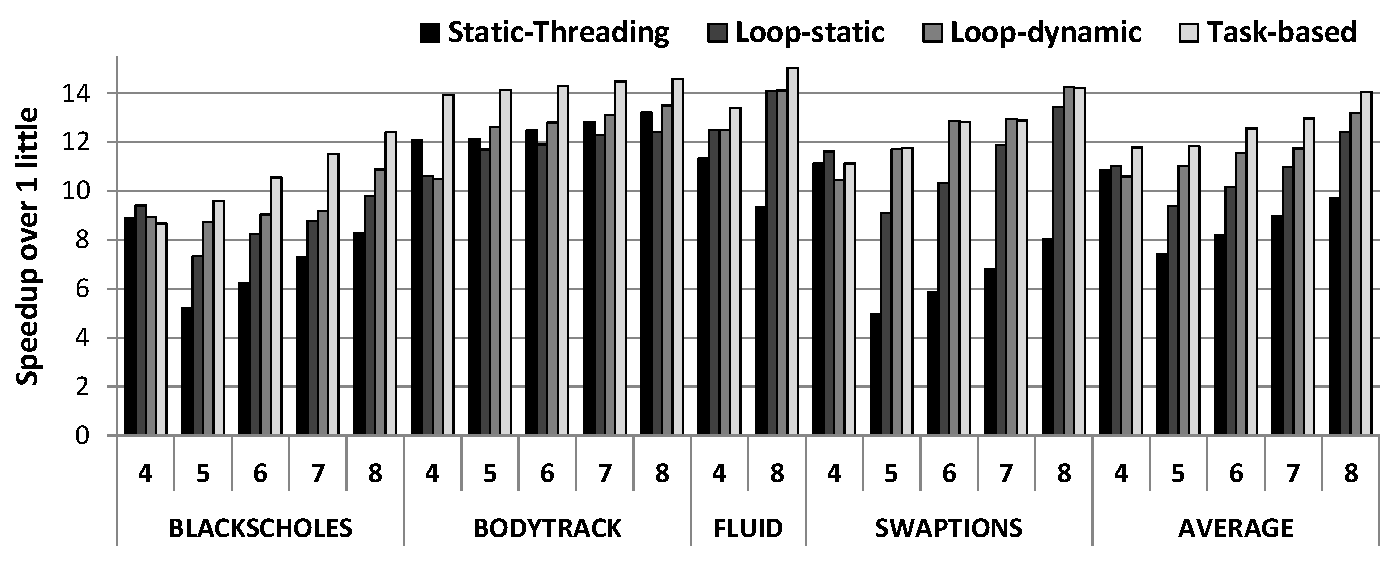
\includegraphics[width=\columnwidth]{figures/speedup-ompssVSopenmp_new}
        \vspace{-0.5cm}
        \caption{Speedup over 1 little core when running on 4 to 8 cores and 4 of them are big. 
Four different programming models are considered: Static threading using \texttt{pthreads}, 
parallel loops with static scheduling (loop static), parallel loops with dynamic scheduling (loop 
dynamic), and a task-based solution with dynamic scheduling (task-based).}%
        \label{fig:prog_models}%
\end{figure}

As we saw in the previous section, current implementations of parallel applications are not ready to fully take advantage of an AMC system.
Applications that are statically threaded using the low-level \texttt{pthreads} library usually suffer from load imbalance since their implementations assume that the work has to be equally distributed among the available cores. 
Implementing advanced load balancing schemes, such as
work pools, in \texttt{pthreads} requires a significant development effort.

As an alternative, many parallel applications are implemented using loop-based scheduling with the 
OpenMP \emph{parallel for} directives. 
In this case, the runtime library is in charge of scheduling work to the available threads in the system, either statically or dynamically, as described in Section~\ref{sec:runtime}.

We compare these solutions to the task-based approach evaluated in the previous sections. 
%Our goal is to evaluate the suitability of each programming model for asymmetric multi-cores. 
Figure~\ref{fig:prog_models} shows the results obtained from running blackscholes, bodytrack, fluidanimate and swaptions on all the scheduling models: static threading, static loop scheduling, dynamic loop scheduling and task-based scheduling. 
We chose these applications as they are the only ones implemented using the OpenMP loop directives.
%available in all the programming models under evaluation: \texttt{pthreads}, OpenMP loop directives and OpenMP tasks.

Looking at the average results in Figure~\ref{fig:prog_models}, we can observe that the task-based solution 
achieves the best results when the system is asymmetric. Task-based improves the static 
threading by up to 59\% on 5 cores, while dynamic loop scheduling improves by up to 54\%.
The OpenMP version with static scheduling reaches an average 26\% improvement over the static-threading approach with pthreads. 
\textcolor{blue}{
\textbf{R1Q12:} The main reason for this improvement is that the OpenMP programming model by default allows the OS scheduler to migrate threads to cores. 
Thus, in this case, GTS is allowed to move threads from little to big cores or vice versa, which differs to the static threading that pins the threads to the cores.
Similarly, loop-dynamic allows dynamic iteration scheduling as well as thread scheduling by GTS.
}

Taking a closer look to the results we observe that for bodytrack, an application with sophisticated parallelization techniques, static-threading achieves better results than loop-static.
This is because the static-threading implementation contains specific parallelization techniques that cannot be completely expressed using the loop-static method.
The loop-dynamic method improves performance for bodytrack by up to 4\% due to the runtime decisions of the iteration execution, but the optimal solution is offered by the task-based approach that achieves up to 16\% improvement over static-threading, due to the flexibility in expressing irregular parallelization strategies.
  
Blackscholes, fluidanimate and swaptions, consist of independent tasks and are a good fit for loop parallelism. 
The first observation is that all three applications benefit from the loop-static approach on an SMC with 4 big cores. 
Moreover, the task-based approach is still the optimal for blackscholes and fluidanimate, reaching up to 83\% improvement over static threading for 5 cores, while for swaptions both task-based and loop-dynamic are efficient, improving the baseline by up to 2.3$\times$.
%The difference in the characteristics of these applications relies on the task granularity; blackscholes consists of 6400 tasks that are about a hundred times smaller than each one of the 128 tasks of swaptions. 
%We attribute this to the fact that loop-dynamic is used in combination with GTS so this allows for an extra scheduling layer through the OS.
%This shows that loop-dynamic is more efficient on coarse-grained applications.
Finally, fluidanimate, that is also a fine-grained application that consists of 128\,500 tasks, also benefits from the task-based approach. 
For this benchmark, static and dynamic loop scheduling achieve similar performance; this is due to the limited parallelism per parallel region, as the loop-based implementation consists of multiple barriers between small parallel regions, fact that diminishes the effect of dynamic vs static scheduling. 
%Thus, if the loops have a small number of iterations, it makes no difference whether these iterations will be scheduled dynamically or statically as the resulting schedule will be the same.

% AR - this sounds wrong, no runtime activity in OMP static sched iteration distribution - This is because the static-scheduling overheads are inside the optimized OpenMP runtime system instead of the application's code. 


  \iffalse
However, 

The second solution is to transfer the responsibility to the runtime system so it dynamically 
schedules work to different core types based on work progress and core availability. The advantage 
is that the runtime system has knowledge of the application structure and parallel work boundaries 
so it can react with certain level of predictability. We evaluate dynamic scheduling on top of the 
existing work-sharing constructs in the applications with an OpenMP statically-scheduled 
implementation available. This requires code transformation that are straightforward in many cases.

We finally evaluate the impact of using a inherently load-balanced execution model such that of 
task-based programming models. Recent examples~\cite{Ayguade:TPDS2009, OpenMP4.0:Manual2013, 
OmpSs_PPL11, Zuckerman:EXADAPT2011, Bauer.2012.SC, Vandierendonck:PACT2011, Vandierendonck:Hyperq} 
include clauses to specify inter-task dependences and remove most barriers which are the major 
source of load imbalance on AMCs.

Comment new figure: Figure~\ref{fig:prog_models}.
Figure~\ref{fig:prog_models} shows the speedup over one little core of blackscholes, bodytrack and swaptions for task-based and static threading solutions compared to loop scheduling solutions. 
The applications are implemented using the OpenMP 2.0 directives for loop scheduling. 
We compare both dynamic and static loop scheduling and the results show that the task-based approach on average outperforms this programming model.
Bodytrack, that consists of highly sophisticated parallel programming techniques performs better with the task-based model as the freedom of task creation and the specification of dependencies helps on a more efficient implementation. 
On the other hand we can observe different behaviour between the highly parallel benchmarks blackscholes and swaptions.
These two benchmarks consist of independent tasks but they show oppositional benefits in terms of the optimal programming model.
Swaptions consists of 128 tasks each of them taking 100$\times$ more time than the blackscholes tasks. 
Blackscholes on the other hand consists of 6400 tasks. 
So, blacksholes is a more fine grained benchmark that lets the task-based programming model to overcome the overheads and increase performance in return.
The loop scheduling work better when the number of tasks is limited and the parallelization is regular.
\fi

%%%%%%%%%%%%%%%%%%%%%%%%%%%%%%%%%%%%%%%%%%
%%%%%%%%%%%%%%%%%%%%%%%%%%%%%%%%%%%%%%%%%%
\if 0 
\subsection{Power Consumption Analysis over Time}

%To understand in detail some of the behaviours pointed out in the last sections, we provide detailed power measurements during the whole execution of the streamcluster benchmark. 

This section provides a detailed analysis of the power consumption over time for one of the evaluated applications, streamcluster.
We choose this application as an illustrative example of the utilization of the processor resources 
(performance and power) with the different evaluated approaches.
Figure~\ref{fig:streamcluster_consumption_evolution} shows the power samples measured over the 
execution time of streamcluster when running on 8 cores (\texttt{4+4} configuration).
On the left part of the figure we plot the power samples of only the 4 big cores, while on the right part we plot the total power samples of all the big and the little cores.
Both charts contain this information for the three scheduling approaches evaluated in this paper (\emph{Static threading}, \emph{GTS} and \emph{Task-based}).
As expected, all the approaches display the same five execution phases throughout the execution, as this benchmark is processing five large chunks of points.
Seemingly the power samples of the big-core cluster slightly outreach 3W for the \emph{GTS} and \emph{Task-based} approaches, while for \emph{Static threading} they remain close to 1.5W. As shown in Figure~\ref{fig:power4}, steamcluster dissipates 1.2W when running on 4 little cores.
Thus, this proves that the \emph{GTS} and \emph{Task-based} approaches better utilize the big cores and, in contrast, the big cores remain idle for a significant amount of time with the \emph{Static threading} strategy.

On the right of Figure~\ref{fig:streamcluster_consumption_evolution}, where the power samples of the whole chip are plotted, the \emph{Task-based} approach has power samples slightly higher than the \emph{GTS} approach:
with the \emph{Task-based} approach, measured power is around 4.0W, while with \emph{GTS} observed power is around 3.6W.
The main difference between these measurements and the ones on the left chart of the same figure is the power consumption of the little cores. 
Thus we derive that both \emph{GTS} and \emph{Task-based} fully utilize the big cores in the system, but the \emph{Task-based} approach utilizes the little cores better than \emph{GTS}. In contrast, \emph{Static threading} does not take advantage of the computational power of this AMC for the streamcluster benchmark.

Despite the fact that performance and power consumption of the little cores are much smaller than the ones of the big cores, the \emph{Task-based} approach significantly reduces the execution time of streamcluster from 374 seconds to 312 seconds. A more effective usage of the little cores at the cost of slightly higher power consumption leads to these results. This clearly demonstrates the benefits of runtime system-based programming models against thread-based approaches in AMC systems.
\fi
%fully using the little cores is extremely important since the task-based approach reduces execution time from 374 to 312 
%without spending much more power by fully exploiting the little cores.


%Figure~\ref{fig:streamcluster_consumption_evolution} contains the measured power consumption per time when streamcluster runs on the 8 cores of the octodroid platform.
%On the left of figure~\ref{fig:streamcluster_consumption_evolution}, we can see the power consumption of just the big cores and on the right the consumption of the whole chip.
%\mc{We need to understand and explain the power dissipation of what hw components (private caches, cores, ...) is being measured.}
%Measurements are shown for the three parallel strategies considered in this paper: \emph{Static Threading}, \emph{GTS} and \emph{task-based}.
%Interestingly, the three considered strategies display the same 5 execution phases, which is obviously expected.
%In terms of power consumption of just the big cores, we can see how these cores dissipate slightly more than 3 Watts when run streamcluster either with the \emph{GTS} or the \emph{Task-based} approaches.
%The \emph{Static threading} approach makes the big cores to dissipate much less power, around 1.5 Watts. 


%This means that the GTS and the task-based approaches use extensively the big cores and, in contrast, the big cores spend a significant amount of idle time under the static threading regime.

%Right of Figure~\ref{fig:streamcluster_consumption_evolution} shows the power consumption when the whole chip is measured.
%In this scenario, things slightly change since the task-based approach spends more power (around 4 Watts most of the time) than the GTS technique (around 3.6 Watts).

%Since the only difference between these measurements and the ones on top of Figure~\ref{fig:streamcluster_consumption_evolution} is the power consumption of the little cores, we can derive that
%the task-based approach uses the little cores much more intensely than the GTS policy, since these cores dissipate much more
%power under the task-based regime than the GTS one. 


%Despite the fact that performance and power consumption of the little cores are much smaller than the ones of the big cores, fully using the little cores is extremely important since the task-based approach reduces execution time from 374 to 312 without spending much more power by fully exploiting the little cores. 

%These results clearly demonstrate the benefits of task-based programming models against thread-based approaches in asymmetric multi-core systems.

